
\documentclass[a4paper,UKenglish,cleveref, autoref, thm-restate]{lipics-v2021}
%This is a template for producing LIPIcs articles. 
%See lipics-v2021-authors-guidelines.pdf for further information.
%for A4 paper format use option "a4paper", for US-letter use option "letterpaper"
%for british hyphenation rules use option "UKenglish", for american hyphenation rules use option "USenglish"
%for section-numbered lemmas etc., use "numberwithinsect"
%for enabling cleveref support, use "cleveref"
%for enabling autoref support, use "autoref"
%for anonymousing the authors (e.g. for double-blind review), add "anonymous"
%for enabling thm-restate support, use "thm-restate"
%for enabling a two-column layout for the author/affilation part (only applicable for > 6 authors), use "authorcolumns"
%for producing a PDF according the PDF/A standard, add "pdfa"

%\graphicspath{{./graphics/}}%helpful if your graphic files are in another directory

\bibliographystyle{plainurl}% the mandatory bibstyle

\title{Hydra Prime: An Exact Solver for Twin-width} %TODO Please add

% \titlerunning{} %TODO optional, please use if title is longer than one line


\newcommand{\universityOfUtah}{School of Computing, University of Utah, USA}
\author{Yosuke Mizutani}{\universityOfUtah}{yos@cs.utah.edu}{https://orcid.org/0000-0002-9847-4890}{}
\author{David Dursteler}{\universityOfUtah}{u1161522@utah.edu}{https://orcid.org/0009-0000-6471-1504}{}
\author{Blair D. Sullivan}{\universityOfUtah}{sullivan@cs.utah.edu}{https://orcid.org/0000-0001-7720-6208}{}

\authorrunning{Y. Mizutani et al.} %TODO mandatory. First: Use abbreviated first/middle names. Second (only in severe cases): Use first author plus 'et al.'

\Copyright{Yosuke Mizutani, David Dursteler and Blair D. Sullivan} %TODO mandatory, please use full first names. LIPIcs license is "CC-BY";  http://creativecommons.org/licenses/by/3.0/

\ccsdesc[100]{Theory of computation → Graph algorithms analysis} %TODO mandatory: Please choose ACM 2012 classifications from https://dl.acm.org/ccs/ccs_flat.cfm 

\keywords{Twin-width, PACE 2023} %TODO mandatory; please add comma-separated list of keywords

\category{} %optional, e.g. invited paper

\relatedversion{} %optional, e.g. full version hosted on arXiv, HAL, or other respository/website
%\relatedversiondetails[linktext={opt. text shown instead of the URL}, cite=DBLP:books/mk/GrayR93]{Classification (e.g. Full Version, Extended Version, Previous Version}{URL to related version} %linktext and cite are optional

\supplement{
    Code submitted to the competition: \url{https://doi.org/10.5281/zenodo.7996823}.
    Code repository on GitHub: \url{https://github.com/mogproject/twinwidth-2023}
}
%optional, e.g. related research data, source code, ... hosted on a repository like zenodo, figshare, GitHub, ...
%\supplementdetails[linktext={opt. text shown instead of the URL}, cite=DBLP:books/mk/GrayR93, subcategory={Description, Subcategory}, swhid={Software Heritage Identifier}]{General Classification (e.g. Software, Dataset, Model, ...)}{URL to related version} %linktext, cite, and subcategory are optional

%\funding{(Optional) general funding statement \dots}%optional, to capture a funding statement, which applies to all authors. Please enter author specific funding statements as fifth argument of the \author macro.

%\acknowledgements{I want to thank \dots}%optional

%\nolinenumbers %uncomment to disable line numbering

\hideLIPIcs  %uncomment to remove references to LIPIcs series (logo, DOI, ...), e.g. when preparing a pre-final version to be uploaded to arXiv or another public repository

%Editor-only macros:: begin (do not touch as author)%%%%%%%%%%%%%%%%%%%%%%%%%%%%%%%%%%
% \EventEditors{John Q. Open and Joan R. Access}
% \EventNoEds{2}
% \EventLongTitle{42nd Conference on Very Important Topics (CVIT 2016)}
% \EventShortTitle{CVIT 2016}
% \EventAcronym{CVIT}
% \EventYear{2016}
% \EventDate{December 24--27, 2016}
% \EventLocation{Little Whinging, United Kingdom}
% \EventLogo{}
% \SeriesVolume{42}
% \ArticleNo{23}
%%%%%%%%%%%%%%%%%%%%%%%%%%%%%%%%%%%%%%%%%%%%%%%%%%%%%%

\newtheorem{rulex}[theorem]{Rule}

% twin-width
\def\tww{\ensuremath{\textnormal{\textsf{tww}}}}

\def\primetreesolver{\textnormal{\textsf{PrimeTreeSolver}}}
\def\directsolver{\textnormal{\textsf{DirectSolver}}}
\def\branchsolver{\textnormal{\textsf{BranchSolver}}}

\def\lbgreedy{\textnormal{\textsf{LBGreedy}}}
\def\lbcore{\textnormal{\textsf{LBCore}}}
\def\lbsample{\textnormal{\textsf{LBSample}}}
\def\lbseparate{\textnormal{\textsf{LBSeparate}}}

\def\ubgreedy{\textnormal{\textsf{UBGreedy}}}
\def\ubseparate{\textnormal{\textsf{UBSeparate}}}
\def\ublocalsearch{\textnormal{\textsf{UBLocalSearch}}}


\begin{document}

\maketitle

%TODO mandatory: add short abstract of the document
\begin{abstract}
This note describes our submission to the Exact track of PACE 2023:
 \textsc{Twin-width}\footnote{%
\texttt{https://pacechallenge.org/2023/}}.
%
Our solver includes linear-time modular decomposition and
a collection of algorithms to find lower and upper bounds of the twin-width.
%
We incorporated the \textsf{Kissat} SAT solver \cite{biere_gimsatul_2022} as a subroutine
and implemented two novel ideas:
\emph{timeline encoding} and \emph{hydra decomposition}.
%
The timeline encoding is a new data structure to compute the width of a given contraction
sequence, enabling faster local search;
the hydra decomposition is a divide-and-conquer strategy featuring a small vertex separator.
\end{abstract}

\section{Background}
\label{sec:background}

We follow standard graph-theoretic notation (e.g. found in \cite{diestel2017graph}),
the original definition of twin-width \cite{bonnet_twin-width_2020,bonnet_twin-width_2021,
bonnet_twin-width_2021-1},
and terminology introduced by Schidler and Szeider \cite{schidler_sat_2021}.
%
Refer to \cite{habib_survey_2010} and \cite{tedder_simple_2008} for the definitions of
a \emph{modular}, \emph{modular decomposition}, a \emph{prime} graph, etc.

We write $(u,v)$ when vertex $v$ is contracted into vertex $u$.
Given a trigraph $G$, the \emph{weak red potential} of $u,v \in V(G), u \neq v$
is the red degree of $u$ after contraction $(u,v)$.
%
We further define
$\triangle(u,v) := N(u) \triangle N(v) \setminus \{u,v\}$ for vertices $u,v$,
where $\triangle$ denotes the symmetric difference of two sets.
%
%
%
%
% A trigraph $G$ is a generalization of an ordinary graph, having vertices $V(G)$ and
% disjoint \emph{black edges} $E_B(G)$ and \emph{red edges} $E_R(G)$.
% %
% We write $G' \gets G / (u,v)$ for contracting
% a vertex $v$ into another (not necessarily adjacent) vertex $u$ in a trigraph $G$
% and resulting in another trigraph $G'$.
%
% A \emph{module} of a graph $G$ is a nonempty set $M \subseteq V(G)$ such that
% for any $x,y \in M$ we have $N(x) \setminus M = N(y) \setminus M$.
% %
% A graph is \emph{prime} if all maximal modules are \emph{trivial},
% i.e. $M=V(G)$ or $|M|=1$.
% %
% The \emph{modular decomposition} of a graph $G$ is given by a rooted tree
% representing the hierarchy of maximal modules.
% %
% Its leaves are individual vertices,
% and internal nodes are called \emph{parallel} if its children are components,
% \emph{series} if its components are co-components, and \emph{prime} otherwise.
% %
% At a prime node, we can obtain a prime graph if we take a quotient graph on the maximal modules.
% %
% Every graph has a unique modular decomposition \cite{habib_survey_2010}.
%
We utilize the following known facts extensively in our implementation.
\begin{itemize}
    \item If $G'$ is an induced subgraph of a graph $G$, then $\tww(G') \leq \tww(G)$ \cite{bonnet_twin-width_2020}.
    \item If $\overline{G}$ is the complement graph of a graph $G$, then $\tww(G) = \tww(\overline{G})$ \cite{bonnet_twin-width_2020}.
    \item $\displaystyle \tww(G) = \max_{H \in \mathcal{P}} \tww(H)$,
    where $\mathcal{P}$ is a set of prime graphs found in the modular decomposition of $G$ \cite{schidler_sat_2021}.
    \item For a graph $G$, $\displaystyle \min_{u,v\in V(G), u \neq v}|\triangle(u,v)| \leq \tww(G)$ \cite{schidler_sat_2021}.
    \item If every component of a graph $G$ has at most one cycle, then $\tww(G) \leq 2$ \cite{ahn_bounds_2022}.
    \item For a tree $T$, $\tww(T) \leq 1$ if and only if $T$ is a caterpillar\footnote{%
    A \emph{caterpillar} is a tree containing a path $P$ such that all other vertices are
    adjacent to some vertex in $P$.
    } \cite{ahn_bounds_2022}.
\end{itemize}


% \subsection{Use of SAT Solver}

% Recent PACE challenges have shown that modern SAT solvers are quite powerful
% to tackle NP-hard graph problems.
% %
% \textsc{Twin-width} is not an exception.
% %
% We adopted a known SAT encoding by Schidler and Szeider \cite{schidler_sat_2021}
% with a few additional clauses.
% %
% Further we employed a SAT solver for finding theoretical lower bounds (\lbcore)
% and finding a vertex separator (\lbseparate, \ubseparate).

% Our code includes the \textsf{Kissat} SAT solver 3.0.0 \cite{biere_gimsatul_2022}
% as an external library, and
% %
% we implemented the sequential counter \cite{sinz_towards_2005} for encoding cardinality constraints.
% Empirically, it performed better than the iterative totalizer \cite{martins_incremental_2014}.

\begin{figure}[t!]
    \centering
    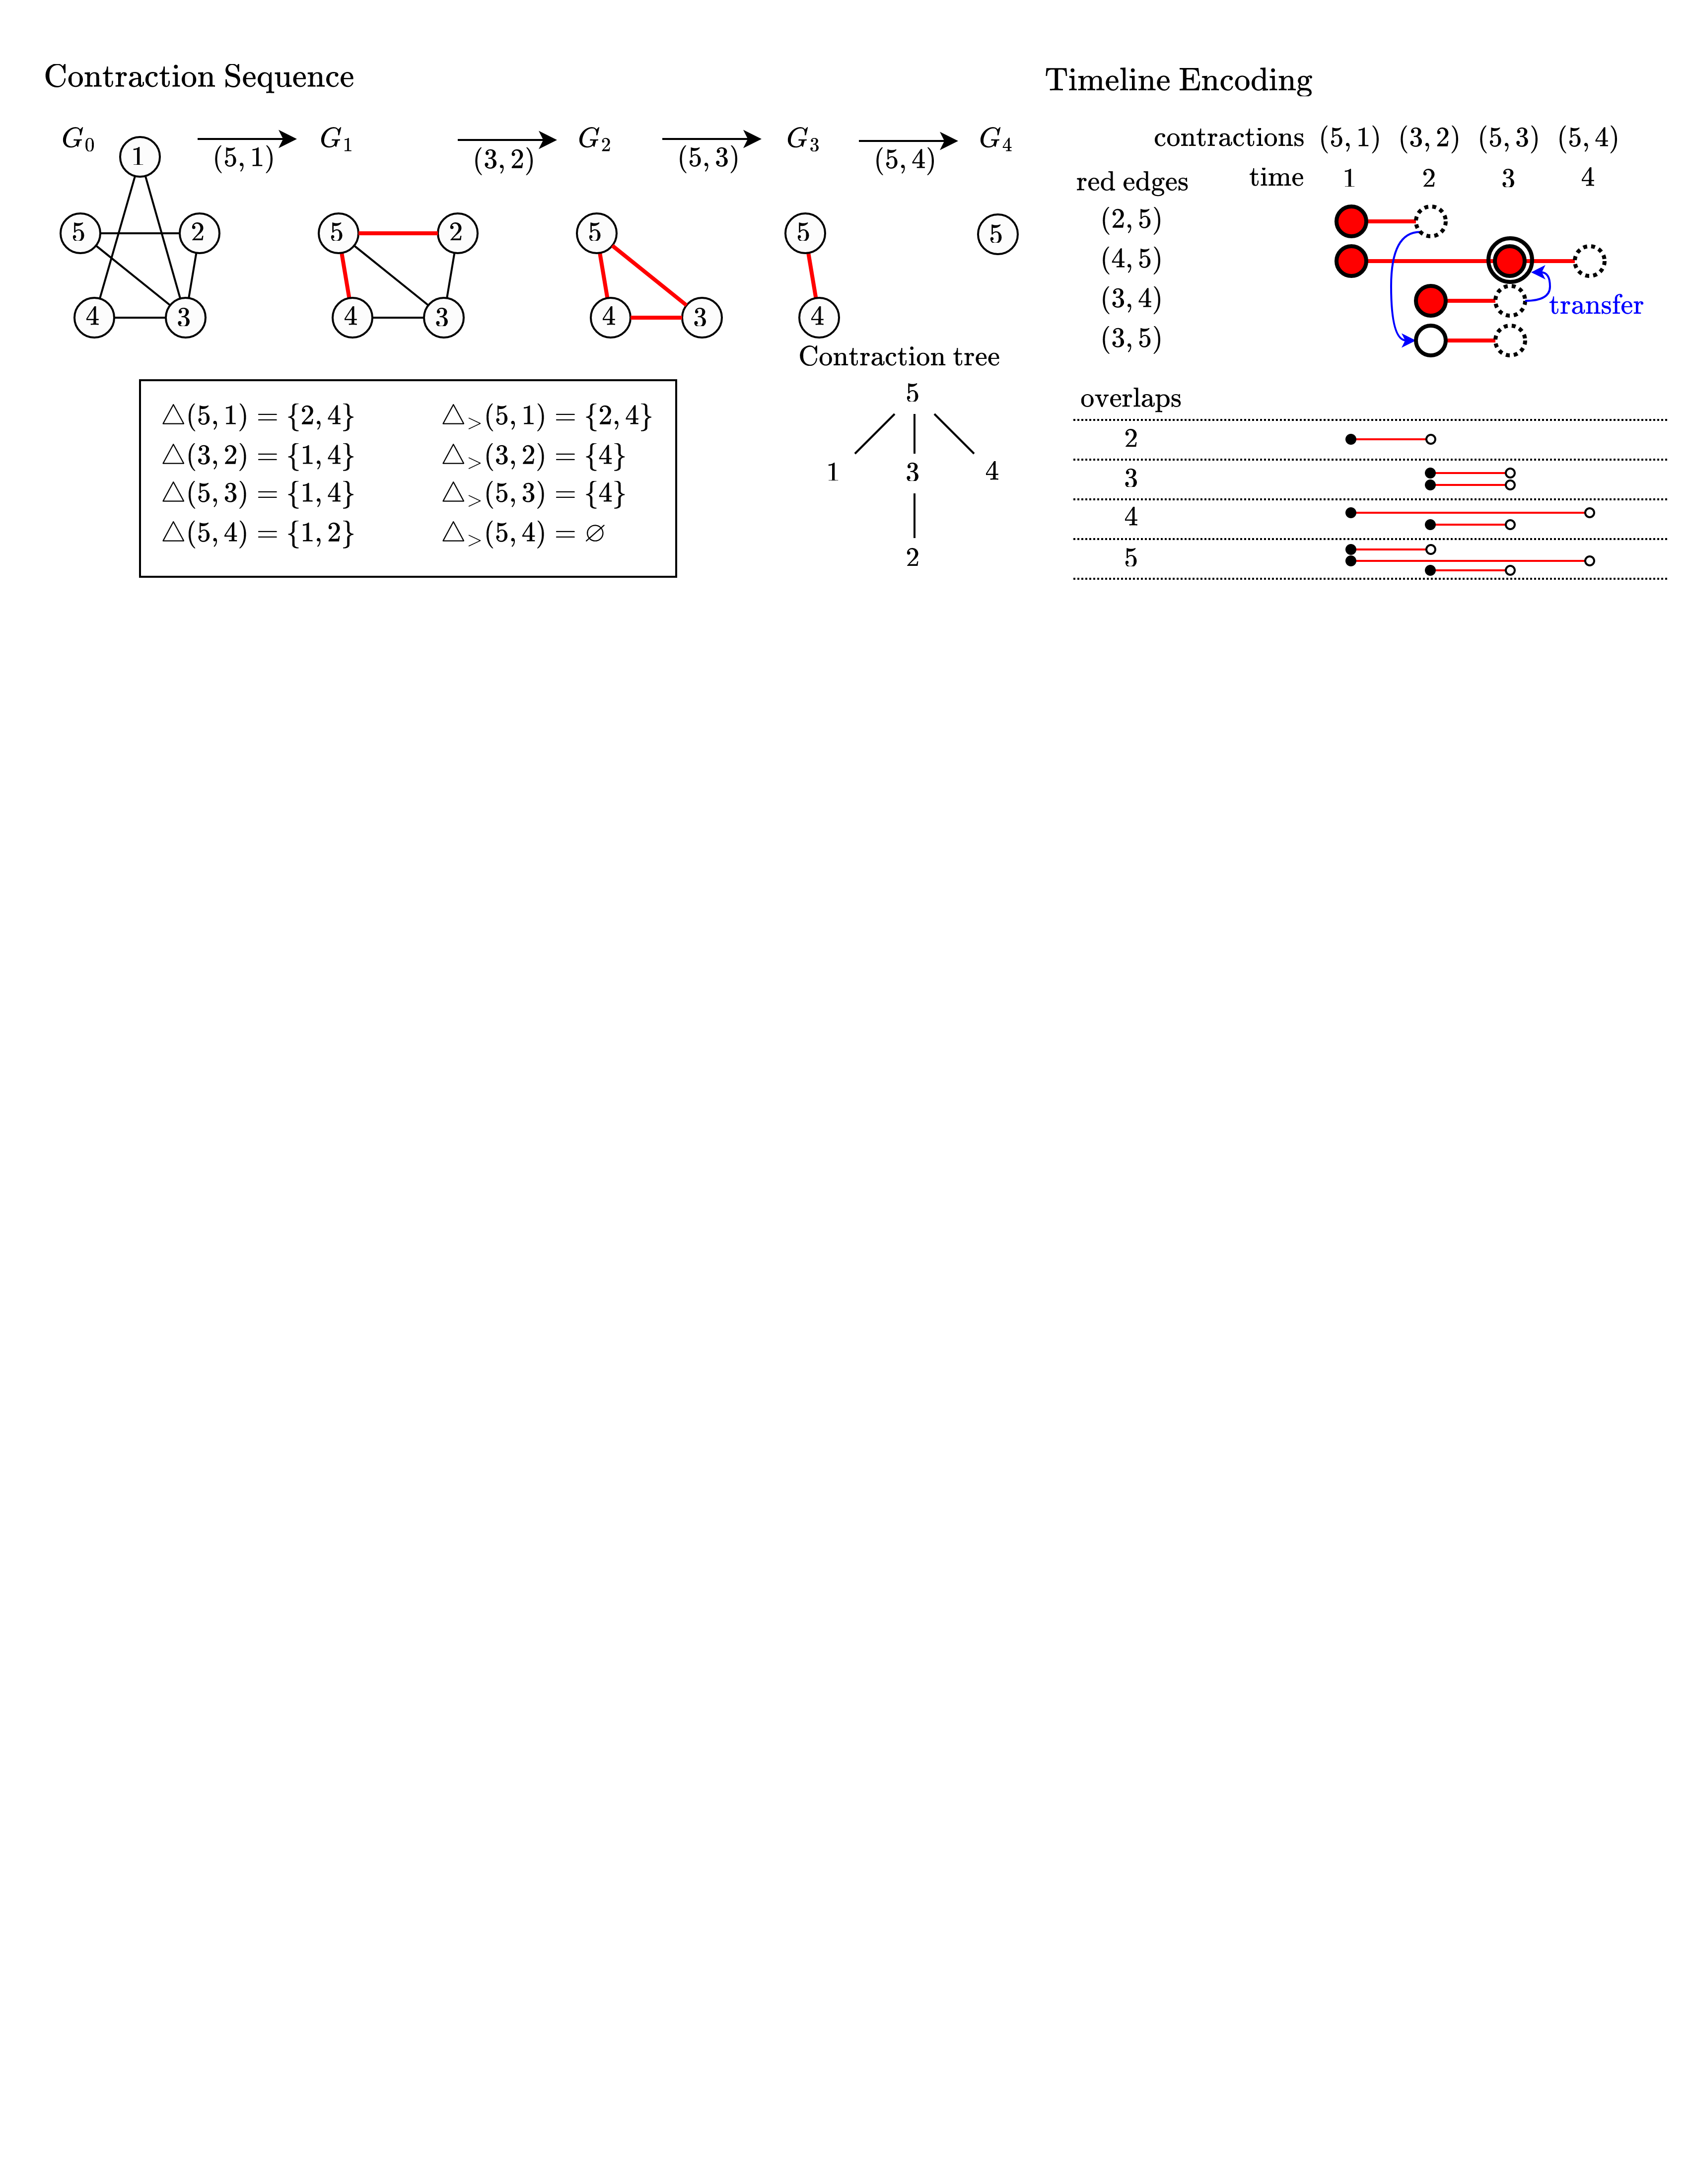
\includegraphics[clip,width=1.0\textwidth,trim={80 3200 80 0}]{images/timeline.png}
    \caption{An example of the timeline encoding,
    along with the given contraction sequence and its contraction tree.
    The red sources are
    $(2,5), (4,5)$ at time $1$, $(3,4)$ at time $2$, and $(4,5)$ at time $3$,
    which creates red intervals
    $[1,2)$ for edge $(2,5)$,
    $[2,3)$ for edge $(3,5)$ (transferred),
    $[1,4)$ for edge $(4,5)$, and
    $[2,3)$ for edge $(3,4)$.
    The red degree corresponds to the number of overlaps of red intervals aggregated by
    vertices, and its maximum (the width of the contractions) is $2$.
    }
    \label{fig:timeline} 
\end{figure}

\section{Timeline Encoding}

In this work we developed the \emph{timeline encoding}, a data structure to 
compute the width of a given contraction sequence.
An instance of the timeline encoding stores the following data.

\begin{itemize}
    \item $G$: input graph with $n$ vertices.
    \item $\phi: V(G) \to [n]$: bijection that encodes an elimination ordering
    (vertex $v$ is eliminated at time $\phi(v)$ if $\phi(v)<n$).
    We write $[n]$ for $\{1,\ldots,n\}$.
    \item $p: [n - 1] \to [n]$: encoding of a contraction tree.
    For $i<j$, $p(i)=j$ if vertex $\phi^{-1}(i)$ is merged into vertex $\phi^{-1}(j)$
    (i.e. $j$ is the \emph{parent} of $i$ in the contraction tree).
\end{itemize}

For internal data structures, we introduce a few terms.
%
First, define $\triangle_{>}(j,i)
:= \{\phi(w) \mid w \in \triangle(\phi^{-1}(i), \phi^{-1}(j)), \phi(w) > i\}$.
%
Then, the \emph{red sources} at time $t$ is a set of red edges
introduced at time $t$, defined as:
$\{\{p(t), k\} \mid k \in \triangle_{>}(p(t), t)\}$.
%
Red sources determine the \emph{red intervals},
non-overlapping, continuous intervals where an edge is red, defined as follows:
%
for $i<j$, red source $(i, j)$ at time $t$ creates an interval $[t,i)$
(red edge $ij$ disappears at time $i$).
If $p(i) \neq j$, then we recurse this process as if red source $\{p(i), j\}$ was created
(red edge $ij$ transfers to $\{p(i),j\}$),
as illustrated in \Cref{fig:timeline}.

Now we aggregate red intervals by vertices.
%
We maintain a \emph{multiset} of intervals for each vertex
such that a red interval of an edge accounts to its both endpoints.
%
The maximum number of the overlaps of such intervals gives
the maximum red degree at a vertex over time.
%
Finally, we obtain the width of the contraction sequence by
taking the maximum of the red degrees over all vertices.
%
A key observation is that we can dynamically compute the number of overlaps of a multiset of
intervals efficiently with a balanced binary tree
(e.g. modification in time $\mathcal{O}(\log n)$,
getting the maximum number of overlaps in $\mathcal{O}(1)$, etc.).
%
For local search, we implemented methods for modifying a contraction tree
and also updating a bijection $\phi$.

\begin{figure}[t!]
    \centering
    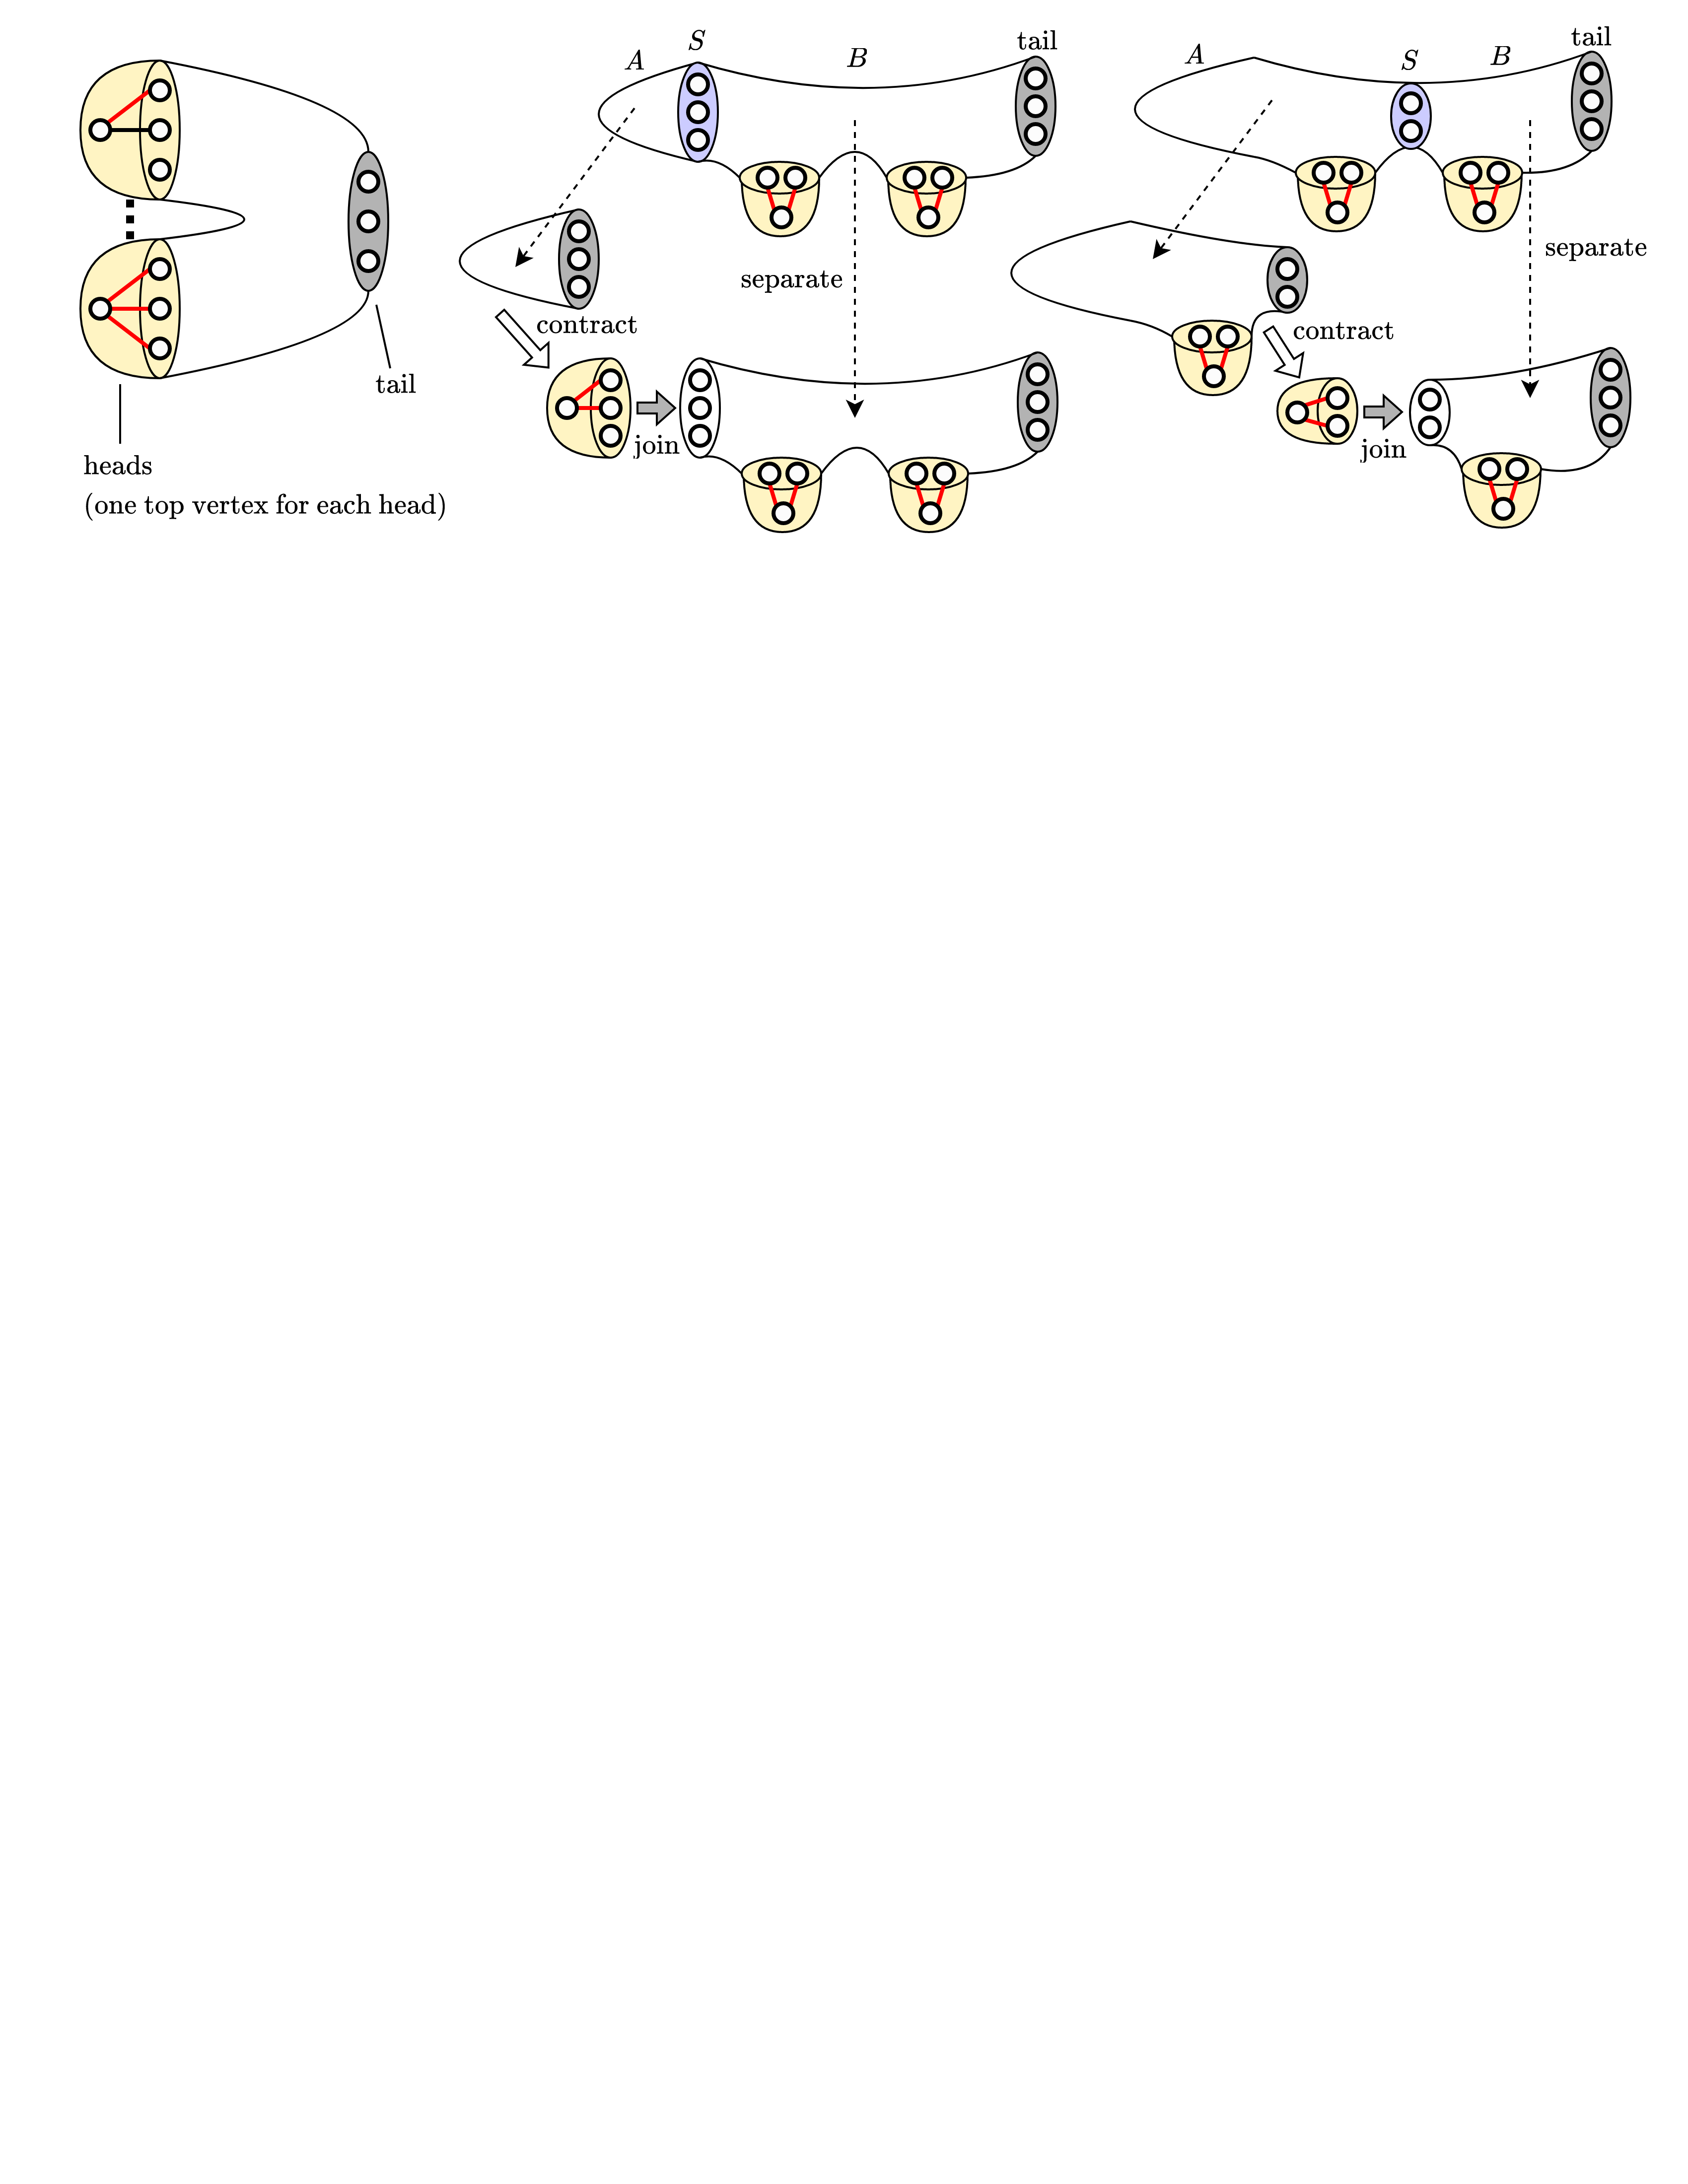
\includegraphics[clip,width=1.0\textwidth,trim={80 3300 80 0}]{images/decomp.png}
    \caption{Structure of the hydra (left) and
    two examples of separating it into two parts (right).
    }
    \label{fig:decomp} 
\end{figure}

\section{Hydra Decomposition}

We also implemented a divide-and-conquer strategy \emph{hydra decomposition},
based on finding a small vertex separator.
%
First, define a structured trigraph, the \emph{hydra},
which consists of a (possibly empty) set of \emph{heads} and
a (possibly empty) vertex set \emph{tail}.
%
Each head contains one \emph{top vertex} and a nonempty set of \emph{boundary vertices}.
The neighbors of the top vertex must be a subset of the boundary vertices.
All red edges in the trigraph must be incident to one of the top vertices.
Heads must be vertex-disjoint, but tail may contain vertices from boundary vertices
(but not a top vertex).

Then, consider partitioning the vertices of a hydra $H$ into three parts:
$S, A, B$ such that $S$ separates $A$ from $B$.
% , i.e. there is no $S$-avoiding path from
% any vertex in $A$ to any vertex in $B$.
%
We also require that $S$ does not contain any vertices from the heads,
and every vertex in the tail must be in either $S$ or $B$.
%
\Cref{fig:decomp} shows two ways of choosing a separator (shaded in light blue)
of a hydra.

Notice that $H[A \cup S]$ is seen as another hydra with $S$ being its tail.
If we contract all vertices of a hydra except the tail,
we will have one vertex ($x$) left and possibly red edges ($E_x$) emanating from it.
%
We then take the rest of the trigraph with vertex $x$, i.e. $H[B \cup S \cup \{x\}]$,
and reattach $E_x$ to it.
Now $x$ and $S$ forms a new head, and we can build up the contraction sequence.
%
As red edges reside only in heads,
if the size of separators are bounded by $d$,
the red degree of a hydra is also upper-bounded by $d$,
which helps construct a $d$-contraction sequence part by part.
%
For $d=1$ we use a linear-time algorithm to find a vertex separator,
or a cut vertex (articulation point).
For $d \geq 2$, we call a SAT solver to find such ones.

\section{Algorithms}

At a high level, the solver first performs linear-time modular decomposition \cite{tedder_simple_2008},
and processes each prime graph.
%
If the prime graph is a tree
% (since every prime graph is connected,
% it is enough to check if the number of edges is less than the number of vertices),
we run \primetreesolver.
%
Otherwise, we run lower-bound and upper-bound algorithms alternatively
until the bounds match.
%
The following is a brief description of each algorithm ((*): using a SAT solver).

\begin{itemize}
    \item Exact algorithms
    \begin{itemize}
        \item \primetreesolver : Linear-time exact solver for trees without twins.
        \item \branchsolver : Brute-force solver equipped with caching mechanism and reduction rules.
        \item \directsolver (*): SAT-based solver implementing the relative encoding presented in \cite{schidler_sat_2021}.
    \end{itemize}
    \item Lower-bound algorithms
    \begin{itemize}
        \item \lbgreedy : Greedily removes a vertex $u$ from the graph $G$
        such that $|\triangle(u,v)|$ is minimized for some $v$.
        Reports the maximum value of $\displaystyle \min_{u,v \in V(G), u \neq v} |\triangle_{G} (u,v)|$.
        \item \lbcore (*): SAT-based algorithm to find 
        $\displaystyle \max_{S \subseteq V(G)} \min_{u,v \in S, u \neq v} |\triangle_{G[S]} (u,v)|$.
        \item \lbsample : Sampling-based algorithm.
        Finds a connected induced subgraph $G'$ of $G$
        by random walk and computes the exact or lower-bound twin-width of $G'$.
        \item \lbseparate (*): Similar to \lbsample, but uses the hydra decomposition to
        find an induced subgraph to check for the lower-bound.
    \end{itemize}
    \item Upper-bound algorithms
    \begin{itemize}
        \item \ubgreedy : Iteratively contract a vertex pair minimizing the weak red potential.
        % We add some randomness in later iterations.
        \item \ublocalsearch : Using the timeline encoding, we make small changes to
        the elimination ordering and the contraction tree to see if there is a better solution.
        \item \ubseparate (*): Divide-and-conquer algorithm using the hydra decomposition.
    \end{itemize}
\end{itemize}

% \footnote{%
% If there are multiple prime graphs,
% we process from the largest to the smallest.
% Larger graphs tend to have a larger twin-width,
% and once we obtain a large lower-bound,
% we can efficiently process the rest of the original graph.
% }.


% We employed the following basic reduction rules.

% \begin{itemize}
%     \item Any contraction is safe if $|V(G)| \leq \tww(G) - 1$.
%     \item A contraction is safe if it does not introduce any new red edges.
% \end{itemize}

%%
%% Bibliography
%%

%% Please use bibtex, 

\bibliography{description}

\end{document}
